% Copyright (c) 2014,2016,2018 Casper Ti. Vector
% Public domain.

\chapter{结论和展望}

\section{分析分析与改进}

\subsection{网络训练结果}
\noindent

使用了如上网络,以100大小的batch进行了50000次训练。训练集共有含过采样的100万张单词图片,测试集为无过采样的1万张单词图片。测试结果评估采用了4个指标,accuracy、precision、recall、F1 Measure。TP为预测正确的正类,FP为预测错误的正类,TN为预测正确的负类,FN为预测错误的负类。accuracy为所有图片预测正确的概率,precision为预测为正类的图片中预测正确的比例,recall为所有正类中被预测正确的比例,F1为precision和recall的调和平均。
\[accuracy = \frac {TP + TN} {TP + FP + TN + FN}\]
\[precision = \frac {TP} {TP + FP}\]
\[recall = \frac {TP} {TP + FN}\]
\[F_1 = \frac {2 TP } {2 TP + FP + FN}\]



在训练集的4个不同位置取一万张图片,以及在测试集上分别计算accuracy、precision、recall、F1 Measure,结果如下表。使用formula\_find.py进行实际效果查看,错误率较高的在于一些短单词,如the、and、of等。对于被分割的公式,在重建时直接将相邻的被预测为公式的单词合并起来,然后用红框标注。发现在测试集上precision明显下降,因为测试集没有过采样,所以非公式图片比公式图片多很多,故有更大比例的非公式图片被识别为公式图片,故precision下降了。也有可能是训练结果过拟合导致的。

\begin{figure}[hp]
\centering
\begin{tabular}{ccccc}
\toprule
Set& accuracy& precision& recall& F1\\
\midrule
Train set 1& 0.83& 0.88& 0.76& 0.82\\
Train set 2& 0.84& 0.87& 0.80& 0.83\\
Train set 3& 0.80& 0.90& 0.67& 0.77\\
Train set 4& 0.79& 0.88& 0.69& 0.78\\
Test set& 0.83& 0.47& 0.72& 0.57\\
\bottomrule
\end{tabular}
\end{figure}

每1000次训练将模型在测试集上进行检测,得到accuracy、precision、recall、F1 Measure的变化趋势。除最开始明显上升外,整体有波动,稳定在一定范围内。

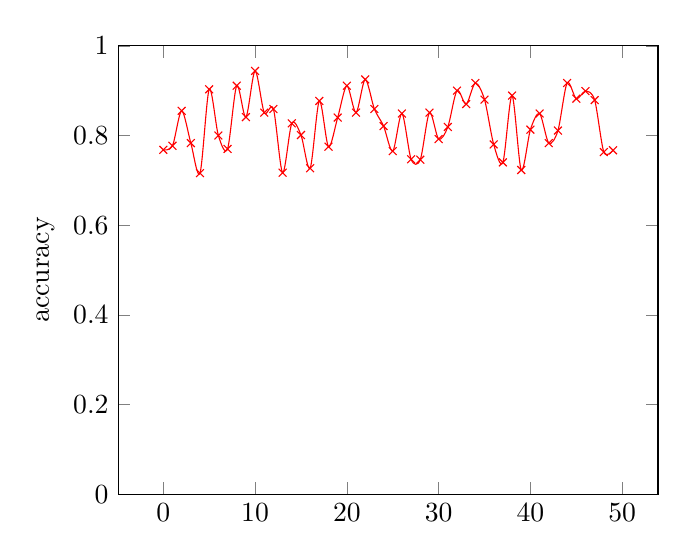
\begin{tikzpicture}
    \begin{axis}[ymin=0, ymax=1,
        ylabel=accuracy]
    \addplot+[smooth, color=red, mark=x]                    % 设置绘图的类型是光滑线图
    coordinates
    {
        (0, 0.7680000066757202) (1, 0.7770000100135803) (2, 0.8550000190734863) (3, 0.7829999923706055) (4, 0.7160000205039978) (5, 0.902999997138977) (6, 0.800000011920929) (7, 0.7699999809265137) (8, 0.9110000133514404) (9, 0.8410000205039978) (10, 0.9440000057220459) (11, 0.8510000109672546) (12, 0.859000027179718) (13, 0.7170000076293945) (14, 0.8270000219345093) (15, 0.8009999990463257) (16, 0.7269999980926514) (17, 0.8769999742507935) (18, 0.7749999761581421) (19, 0.8399999737739563) (20, 0.9110000133514404) (21, 0.8510000109672546) (22, 0.925000011920929) (23, 0.859000027179718) (24, 0.8209999799728394) (25, 0.7649999856948853) (26, 0.8489999771118164) (27, 0.746999979019165) (28, 0.7459999918937683) (29, 0.8510000109672546) (30, 0.7919999957084656) (31, 0.8190000057220459) (32, 0.8999999761581421) (33, 0.8700000047683716) (34, 0.9169999957084656) (35, 0.8799999952316284) (36, 0.7799999713897705) (37, 0.7400000095367432) (38, 0.8889999985694885) (39, 0.7229999899864197) (40, 0.8130000233650208) (41, 0.8489999771118164) (42, 0.7829999923706055) (43, 0.8109999895095825) (44, 0.9169999957084656) (45, 0.8820000290870667) (46, 0.8989999890327454) (47, 0.8790000081062317) (48, 0.7630000114440918) (49, 0.7670000195503235)
    };
    \end{axis}
\end{tikzpicture}


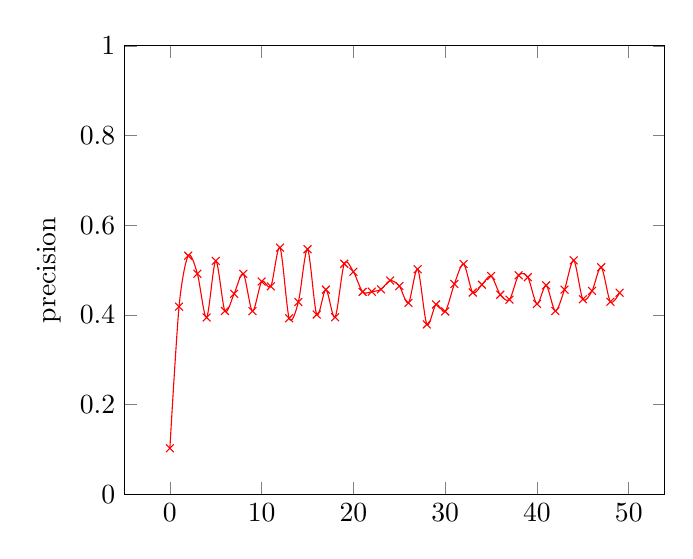
\begin{tikzpicture}
    \begin{axis}[ymin=0, ymax=1,
        ylabel=precision]
    \addplot+[smooth, color=red, mark=x]                    % 设置绘图的类型是光滑线图
    coordinates
    {
        (0, 0.10227267450940637) (1, 0.4181817318844488) (2, 0.531791767957752) (3, 0.4914528961028762) (4, 0.39402169052022534) (5, 0.5202701106741453) (6, 0.40856023911048184) (7, 0.44680845668863683) (8, 0.4913791180295048) (9, 0.4080716658007849) (10, 0.4742265821664585) (11, 0.4634145315171357) (12, 0.5497834417310405) (13, 0.3923705236686806) (14, 0.42857135344745423) (15, 0.546255397357019) (16, 0.4005681301540768) (17, 0.45614022977348306) (18, 0.39455776220103844) (19, 0.5138888078801535) (20, 0.4959998198531441) (21, 0.45116269542904797) (22, 0.4516127378775276) (23, 0.45673066954067154) (24, 0.4763778676081821) (25, 0.4641743891791755) (26, 0.42672405442568057) (27, 0.5015872292951588) (28, 0.3786126670838483) (29, 0.42307683073241154) (30, 0.4074073389027238) (31, 0.46885238922667033) (32, 0.5133331779647318) (33, 0.44973534170395274) (34, 0.4671531298633628) (35, 0.4864863372537463) (36, 0.44478521413123473) (37, 0.43380276142362) (38, 0.48809510619355034) (39, 0.4838709033205131) (40, 0.4242423512857085) (41, 0.46575332810425396) (42, 0.40845063893087913) (43, 0.4560810111282234) (44, 0.5214284023370511) (45, 0.43478248609258174) (46, 0.4534160212108353) (47, 0.5060239579912521) (48, 0.4289854507944657) (49, 0.4491017353617148)
    };
    \end{axis}
\end{tikzpicture}

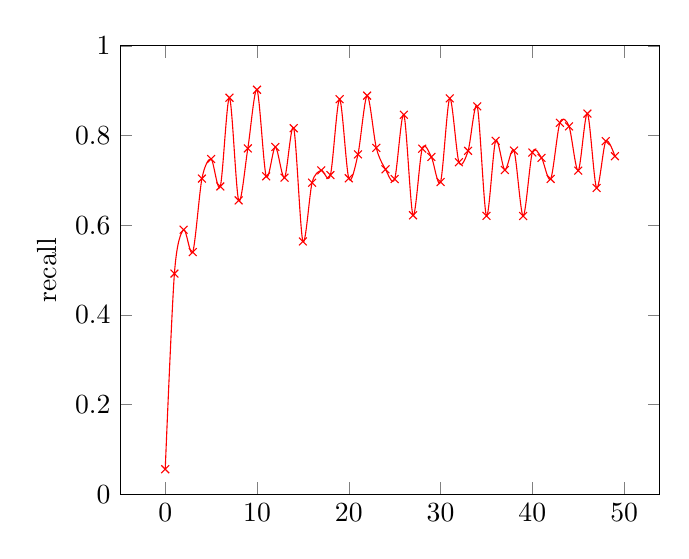
\begin{tikzpicture}
    \begin{axis}[ymin=0, ymax=1,
        ylabel=recall]
    \addplot+[smooth, color=red, mark=x]                    % 设置绘图的类型是光滑线图
    coordinates
    {
        (0, 0.05555553998631103) (1, 0.49197849018294704) (2, 0.5897434181133989) (3, 0.5399059882080096) (4, 0.7038833400181834) (5, 0.7475724860219577) (6, 0.6862743061646712) (7, 0.8842103150363884) (8, 0.6551720718992409) (9, 0.771186143967824) (10, 0.9019599813937293) (11, 0.7089549836827875) (12, 0.7743900295289454) (13, 0.7058821958480288) (14, 0.8161761981298377) (15, 0.5636362473225179) (16, 0.6945811254485994) (17, 0.7222219186219965) (18, 0.7116562435021873) (19, 0.88095214288592) (20, 0.7045450910647995) (21, 0.75781223121389) (22, 0.8888882483259677) (23, 0.7723574384961508) (24, 0.7245507012302338) (25, 0.7028300381677623) (26, 0.8461535178178609) (27, 0.6220471329098577) (28, 0.7705880295021034) (29, 0.752136460282543) (30, 0.6962023315978674) (31, 0.8827158020047197) (32, 0.7403842921788956) (33, 0.7657654525612815) (34, 0.8648643342597293) (35, 0.6206894122477955) (36, 0.7880432838200557) (37, 0.723004540730726) (38, 0.7663548150237872) (39, 0.6203006460090009) (40, 0.7619045265958367) (41, 0.7499997496328238) (42, 0.7030301095908024) (43, 0.8282206282137524) (44, 0.8202243006952176) (45, 0.7216491467750457) (46, 0.8488367611961705) (47, 0.6829265771965964) (48, 0.787233852444885) (49, 0.7537686722560564)
    };
    \end{axis}
\end{tikzpicture}
    
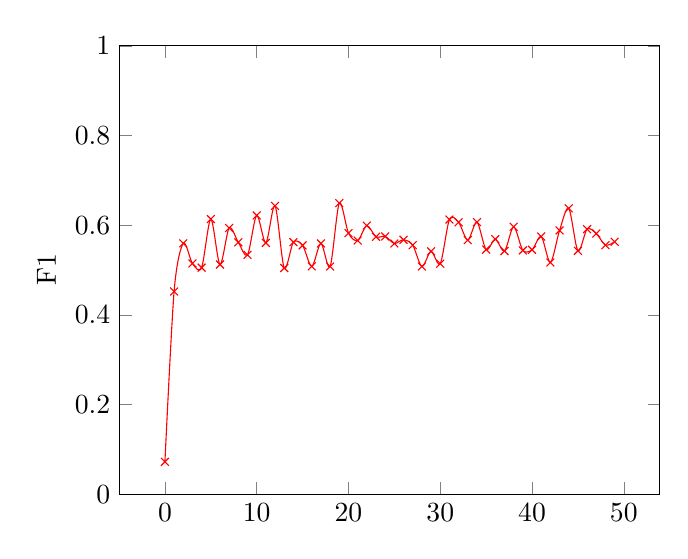
\begin{tikzpicture}
    \begin{axis}[ymin=0, ymax=1,
        ylabel=F1]
    \addplot+[smooth, color=red, mark=x]                    % 设置绘图的类型是光滑线图
    coordinates
    {
        (0, 0.0719999869248226) (1, 0.45208840165901304) (2, 0.5592704395415238) (3, 0.5145413347647865) (4, 0.50522644087588) (5, 0.6135457057572432) (6, 0.5121950652350732) (7, 0.593639528354783) (8, 0.5615762290861016) (9, 0.5337242691171721) (10, 0.6216214309353425) (11, 0.5604719013410473) (12, 0.6430379007749987) (13, 0.504378243609918) (14, 0.5620252518584634) (15, 0.5548097870507263) (16, 0.5081080665440171) (17, 0.5591396939609217) (18, 0.5076585928935132) (19, 0.6491227423900725) (20, 0.5821595003286365) (21, 0.5655975927752449) (22, 0.5989303358748921) (23, 0.5740180481559545) (24, 0.5748217907437793) (25, 0.5590993895251913) (26, 0.5673351697507826) (27, 0.5553602368834522) (28, 0.5077518933102708) (29, 0.5415383858898317) (30, 0.5140186370644626) (31, 0.6124196406770692) (32, 0.6062991042285955) (33, 0.5666665809112568) (34, 0.6066349405631104) (35, 0.5454544516530538) (36, 0.5686274003614823) (37, 0.5422534777847363) (38, 0.5963635379095901) (39, 0.54365729047446) (40, 0.5450121052469311) (41, 0.5746478138338862) (42, 0.5167037339458502) (43, 0.5882352359349926) (44, 0.6375544587557744) (45, 0.5426355634278431) (46, 0.5910930087628296) (47, 0.5813147875721435) (48, 0.5553470446290492) (49, 0.5628517344213336)
    };
    \end{axis}
\end{tikzpicture}

\subsection{分析与改进}
\noindent

网络结果不尽如人意,对于原因有如下分析。

一是在数据上。数据过于简单,特别是过采样部分,直接使用了复制原图片的方式进行过采样,缺乏变化。单词图片之间也有很大差异,寻找共性特征比较困难,故长单词一般很好地被区分,但短单词却容易和公式混淆。而且公式内也有许多字母符号,与某些非公式单词可能难以分别。实际上短单词也容易被误认为是公式,尤其是and、of。对于单词the,在测试时发现同一张论文图片中,有的the被认为是公式,有的被认为是单词,于是将这些the单独提取出来,发现只有图片的高度不同,高度高一点的被认为是公式,高度低一点的被认为是单词,这也是由于数据本身的多样性不足。

二是在参数初始化上,直接使用了截断正态分布来初始化权重,可能会对结果造成影响。

三是网络结构上。这次采用的网络结构主要是根据自身条件进行的舍取,缺乏有效性的验证。

根据以上的错误分析,可以有如下的改进。在数据预处理上,采用最小二乘法的单词分割虽然效果还不错,但还不够精确,特别是容易将公式分割开。不过,如果仍然采用以空格为依据的单词分割,这一点比较难改进,有的公式内部确实有较大的空格,与单词间空格难以区分,但可以尝试精细的调参,提高表现,还可以使用去掉一些较小值后再进行最小二乘法,使结果更偏离小宽度空白。在过采样时,应该使用更多样化的采样,如使用SMOTE算法进行过采样。SMOTE算法是将少数类样本取k临近样本并在两个样本间做一个随机的平移。由于网络使用了spp层,还可以考虑将输入图像resize到更多尺度的数据做多尺度的训练。在参数初始化上,可以采用MSRA初始化,即权值初始化为服从方差为$\frac 2 n$的高斯分布。\cite{msra}网络结构上应该测试更多的模型,并在通过验证集调节超参数,对网络的深度、学习率、核尺寸等进行进一步的调节。